\documentclass[full.tex]{subfiles}


% change this line
\graphicspath{ {assets/note6/} }
\newcommand{\notenum}{6}



\begin{document}
    \thispagestyle{firstpage}
    \vspace*{2\baselineskip}
    \section*{Game Theory \& Network Attacks: How to Destroy Bitcoin}
    
    As with any other distributed network, the Bitcoin network is subject to a variety of attacks. In this note, we will take a closer look at potential attacks that could be used to take down the Bitcoin network. As we will find, destroying Bitcoin is actually fairly simple.
    
    \section*{Mining Pools}
    
    Recall the concept of mining pools, which allow individual miners to combine or `pool,' their computational power together. Mining pools are run by \textbf{pool managers} or \textbf{pool operators}. The pool manager usually takes a cut of the ming rewards first, and the rest is distributed to other nodes in the pool, usually depending on the amount of hash power these nodes offer. As a result, a miner can achieve a relatively stable profit. If the mining pool is large enough, an individual miner in the pool can expect profit from the block reward regularly, in proportion to their own hash power. In contrast, mining alone implies a higher variance in mining rewards; you can expect to not win the block reward the majority of the time, but when you do win, the payout is huge. Mining pools also lower the barrier of entry for new miners, democratizing the mining scene. Instead of having to purchase an array of ASICs, individuals can opt to participate in a mining pool. Additionally, mining pools are easily upgraded, since only the pool manager has to upgrade on behalf of the pool. Everyone else can continue contributing hash power as before.
    
    Although the idea of mining pools might seem enticing for the average miner, mining pools are actually detrimental overall to the health of the Bitcoin network. Mining pools are centralized, around one pool manager, and bring with them the security flaws of centralized systems. For example, the pool manager must be trusted to distribute block reward in a fair manner. Especially as mining pools grow larger, and represent the majority of total hash power, the Bitcoin network may not be as safe as we like to think.
    
    \section*{Mining Pools --- Example}
    
    We will now compare estimated profit for a solo miner versus a miner in a mining pool. Suppose you want to start mining today. The best ASIC on the market, the Antminer S9, costs \$2400, and has an average hash rate of 14 TH/s. Today's (July 21, 2017) total network hashrate is 6,478,893 TH/s. Buying an Antminer S9 would get you $\frac{14~TH/s}{6,478,893~TH/s} = 0.000216086\%$ of the network hashrate. The total amount of mining reward awarded every year is $1~yr * \frac{12.5~BTC}{10~min} = 657,000~BTC/yr$. According to the percentage of network hashrate you own, you would expect to get an annual reward of: $0.000216086\% * 657,000~BTC/yr = 1.42 BTC/yr$. 
    
    However as a solo miner, you can't assume that you will win block reward consistently, with low variance. A more accurate calculation would be to consider the expected number of blocks you will mine, not block reward, proportionate to your hash power. Given the percentage of total hash power you own, you can expect to mine one block every 462,779 blocks. This translates to \textit{one block, 12.5 BTC, every 3214 days (8.8 years)}. This payout is way too infrequent. Now consider the case for mining pools. Assume the mining pool has 1/6th of the network hash rate. The pool would find every 6th block. We simply divide our expected annual reward, based on the proportion of hash power we own, with 8760 hours in a year to get the hourly rate. $1.42~BTC/yr~/~(8760~hr/yr) = 0.000162~BTC/hr$. 
    
    At today's exchange rate, 1 BTC = 2771.92 USD. Solo mining would yield $34,649~USD/8.8~yr$, whereas mining with a large mining pool (assuming the pool has 1/6 of the network hashrate) yields a much more frequent payout of $0.45~USD/hr$. For most, the frequent payout of large mining pools ensures them the maximum profit. This is especially true when one considers the fact that current-day mining hardware will probably be obsolete in 8.8 years anyways, due to increasing network hash power and overall network security. Paradoxically, as Bitcoin gets more secure, the more we need mining pools, whose dangerous centralization dangerously contrasts with Bitcoin's underlying concepts of decentralization.
    
    
    \section*{Mining Pools --- Hash Rate Distribution}

    \begin{center}
        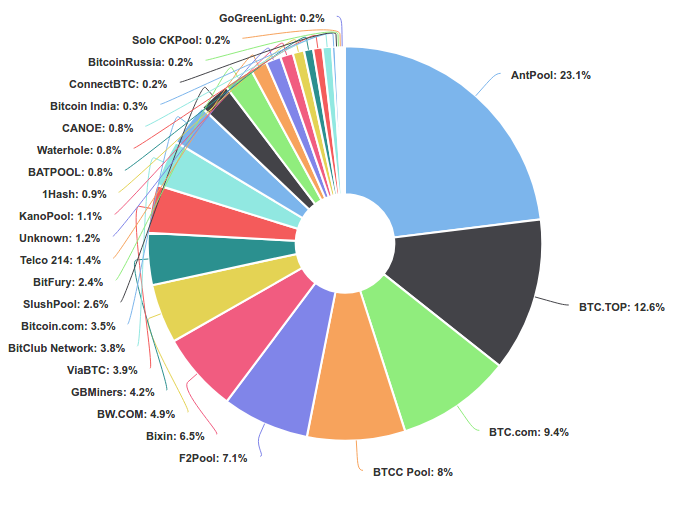
\includegraphics[scale=0.5]{hash_rate_distribution}
    \end{center}
    
    Above is a pie diagram of the mining pool hash rate distribution from \underline{blockchain.info} on July 25, 2017. In general, the Bitcoin community exhibits backlah against large mining pools that gain too much power. In 2014, a large mining pool called GHash.io actually exceeded the 51\% threshold, causing controversy among the Bitcoin community. Miners recognized the economic incentives of joining mining pools, and GHash.io provided the most potentiall for profot. Fortunately, miners voluntarily left the dangerously powerful GHash.io to uphold the health of the network.
    
    One of the most frightening aspects of mining pools is a phenomenon called \textbf{laundering hashes}, a process by which a single entity participates in multiple pools. Laundering hashes are very difficult to detect because it is difficult to detect where new blocks are coming from, and whether they are associated with mining pools. By extension, this raises the concern that the actual concentration of control over mining hardware is \textit{unknown}.
    
    \section*{Mining Pools --- Shares}
    
    For mining pools to distribute the block reward, they must keep track of which miners are in their pool, as well as the proportion of computational power they contribute to the pool. To prove that they actually contribute to the pool, miners submit \textbf{shares}, or ``near-valid'' blocks, to mining pools. Producing shares implies that computational power has been expended to help the pool find the block reward. After a block reward is found, the mining pool operator distributes the reward proportionally to the number of shares submitted, which approximates the proportion of computational power expended.
    
    Valid blocks are also considered shares. A miner who finds a valid block is not rewarded any extra coins from the block reward. This is because the valid block is based on the Merkle root given by the pool operator. The coinbase transaction goes to the pool operator, who redistributes the profit to the pool. In this way, a miner cannot just submit shares in a pool and keep the reward of the valid block for themselves.
    
    \section*{Mining Pools --- Basic Reward Schemes}
    
    There are two basic reward schemes that mining pools employ to reward miners. \textbf{Pay-per-share} is a reward scheme that pays out at every share submitted. Every time a miner submits a share, the pool will pay the miner for their share. Be default, the pay is proportional to the work done. Pay-per-share is beneficial for miners rather than the pool, since individual miners face no risk from reward variance. Instead, it is the pool that has to deal with reward variance, since they only profit when a block reward is found. One major problem of pay-per-share is that there is no incentive for miners to actually submit valid blocks, since miners are paid regardless.
    
    \textbf{Proportional} reward schemes are those that pay out to miners whenever a block is found, proportional to the work that individuals have submitted for the current block. Because individual miners only profit when the entire pool finds a valid block, proportional reward schemes are more beneficial to the pool. Individual miners bear some risk in variance proportional to the size of the pool. They are not paid if a valid block is not found. This is generally not a problem if the mining pool is sufficiently large, and block rewards are fairly consistent. For mining pool operators, proportional reward schemes provide lower risk, since they only have to pay individual miners when a reward is found. In this way, individual miners are incentivized to submit valid blocks, solving the fundamental problem of the pay-per-share reward scheme.
    
    \section*{Pool Hopping}
    
    Because miners seek profit, the existence of multiple mining pool reward schemes gives rise to questionable behavior aimed to maximize profit. \textbf{Pool hopping} is a practice among some miners that involves switching between different mining pools to increase their total profit. This is done in observance of the facts that proportional mining pools pay larger amounts per share if a block is found quickly, and that pay-per-share mining pools pay out regardless, but often times not in as high of quantities as in proportional pools.
    
    An example of a clever strategy that a miner might employ to maximize profits is:
    
    \begin{itemize}
        \item Mine in a proportional pool shortly after a block was found, while rewards are high since there have not been many shares submitted yet.
        \item Switch to a pay-per-share pool once the proportional pool is less profitable, since they always pay out. 
    \end{itemize}
    
        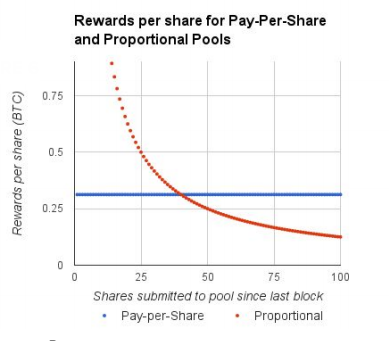
\includegraphics[scale=1]{pool_hopping}
    
    \begin{center}
    \end{center}

    
    In the chart above, we compare the rewards per share for pay-per-share and proportional pools. We take, for sake of an example, that the mining pool has 10\% of the network hash rate, and that we can expect about 4 shares per miner for each valid block.

    The practice of pool hopping is detrimental to the mining pool scene. Honest miners who stay loyal to one mining pool are cheated out of their money, since miners who pool hop submit shares only when it is profitable. Therefore, proportional pools are not feasible in practice. Designing a mining pool reward scheme with aligned incentives , for miners and the pool, that is not vulnerable to pool hopping remains an open problem. 
    
    \section*{Pool Wars}
    
    Let's create a theoretical scenario to simplify some of the calculations we'll be doing in this section. Assume that you have 30\% of the network hash rate, and that the block reward is 1 BTC. Owning 30\% of the hash rate equates to winning 30\% of the mining reward, so on average you would expect to get 0.3 BTC per block. Now, suppose you buy more mining equipment, worth 1\% of the current network hash rate. With a standard mining strategy, adding 1\% network hash rate would mean you now own 30.69\% network hash rate, since $\frac{31}{101} = 30.69\%$. Your revenue gain from 1\% hash rate added would be 0.0069 BTC. 
    
    Instead of deploying the standard mining strategy, say that you decide to \textbf{cannibalize pools}. You distribute your 1\% equally among all other pools, and withhold valid blocks. You would still receive mining pool rewards from the shares you submit. The other pool owns 70\% of the network hash rate still because you are not contributing in its efforts to find a valid block, you are simply diluting it. 70\% network hash rate expects to earn 0.7 BTC per block. You own $\frac{1}{71}$ of the other pool, so your expected value from mining and submitting shares in this other pool would be $\frac{1}{71} * 0.7 = 0.0098~BTC$. Therefore, we can conclude that since 0.0098 BTC > 0.0069 BTC, it is more profitable to cannibalize pools than to mine honestly.
    
    \section*{Selfish Mining (Block-Withholding)}
    
    Instead of withholding a block from a mining pool, what happens when we withhold a block from the entire network? This is malicious mining strategy called \textbf{selfish mining}, or \textbf{block-withholding}. (The terminology can be a bit confusing, since pool cannibalizing is also a form of withholding a block, but in this scenario block-withholding is in the context of the entire network.) Suppose you are a miner and you have just found a block. Instead of announcing the block to the network and receiving a reward, you keep it a secret. You try to find two blocks in a row before the network finds the next one. If you succeed, once you announce this block, you can receive block rewards for both blocks, since you have the longer chain with two blocks that the rest of the network does not have. The image below shows a selfish miner (bottom) two blocks ahead of the rest of the network (top).
    
    \begin{center}
        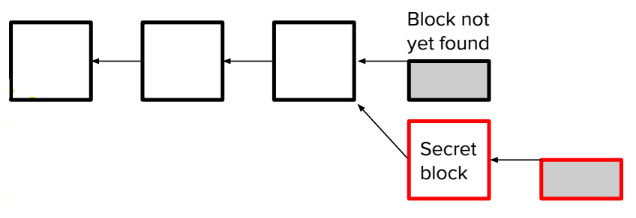
\includegraphics[scale=0.6]{selfish}
    \end{center}
    
    If however your plan fails, and the network finds their new block before you can find a second one, there begins a \textbf{race to propagate}. You and the rest of the network have competing blocks. It is mathematically proven that assuming you have 50\% chance of winning the race and having your block accepted by the network, this malicious strategy of selfish mining is only profitable if you have more than 25\% of the network hash rate. It is also true that if you have more than 33\% of the network hash rate, you can lose the race to propagate every time, and your malicious strategy would still be more profitable. While no one individual probably owns this much of the network hash rate on their own, if a large mining pool (or several) banded together in hopes of increasing their own profits, they could potentially deploy the strategy of selfish mining and profit every time.
    
    \section*{Blacklisting via Punitive Forking}
    
    Say you are a government that has jurisdiction over many mining pools, say China. Your objective is to censor the Bitcoin addresses owned by certain people, say Gary Johnson, and to prevent them from spending any of their bitcoin. How do we censor Gary Johnson from the Bitcoin network? In the following sections, we will analyze some strategies that could be used to blacklist someone from the Bitcoin blockchain. We will use the following types of blocks in our illustrations. 
    
    \begin{center}
        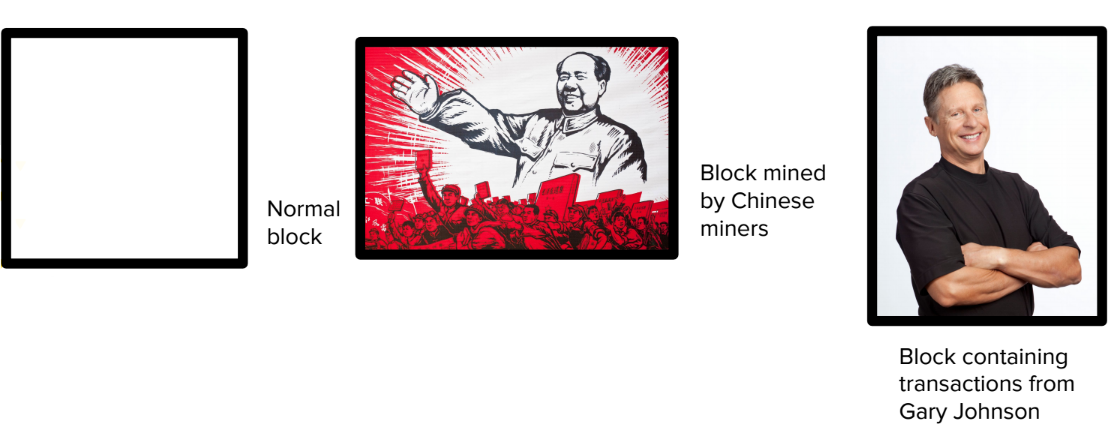
\includegraphics[scale=0.3]{blacklist_block_types}
    \end{center}
    
    Your first strategy might be to tell your country's mining pools to not include any of Johnson's transactions, in a process known as \textbf{blacklisting}. This strategy will not work unless you are 100\% of the network, and you mine all of the blocks, all the time. If you do not have complete control over the network, it is possible that other miners will eventually include Gary Johnson's transactions into a valid block, and propagate that before your country can. This strategy is not a practical way to censor Johnson from the network, and realistically can only cause delays and inconveniences.
    
    \begin{center}
        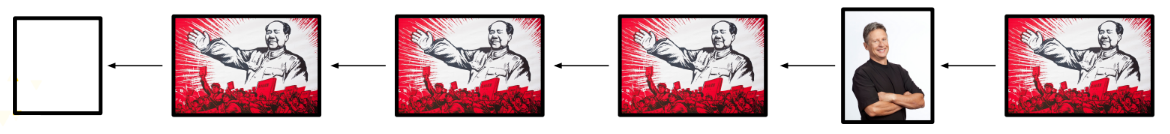
\includegraphics[scale=0.4]{blacklist_punitive}
    \end{center}
    
    You decide to change up your strategy. You are China after all, and you have more than 51\% of the network hash rate, so you mandate that Chinese pools refuse to work on a chain containing transactions spending from Gary Johnson's Bitcoin address. You then announce your blocks to the world as usual. Since you have the majority of the network hash rate, you will always have the longer chain in the long run, and thus you can always invalidate Gary Johnson's transactions whenever you overtake the rest of the network's chain. In other words, if non-Chinese miners include a transaction from Johnson in a block, China will fork and create a longer proof-of-work chain. The non-Chinese block containing Johnson's transactions will be invalidated. 
    
    \begin{center}
        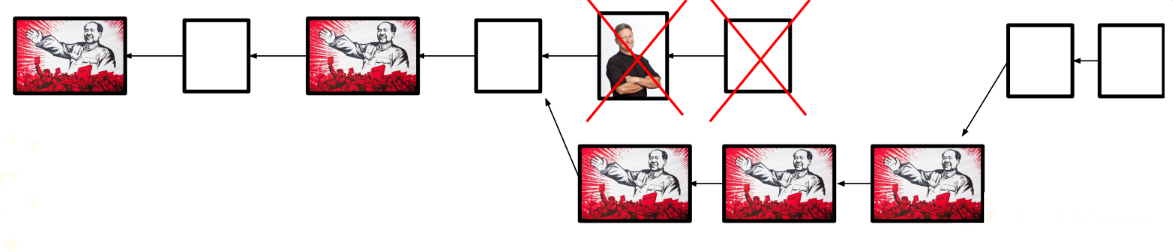
\includegraphics[scale=0.4]{blacklist_punitive2}
    \end{center}
    
    As a result of having their blocks constantly being invalidated, non-Chinese miners would eventually stop trying to include Johnson's transactions when mining blocks. Thus, we have shown how a 51\% majority can prevent anyone from accessing their funds (blacklisting). This particular method of blacklisting is called \textbf{punitive forking}, since you can make a fork in the blockchain, and since you have majority hash rate, everyone else would have no choice but to join your chain, else waste their computing power on a chain that will never win.
    
    \section*{Blacklisting via Feather Forking}
    
    One weakness of punitive forking is that it only works if you have a majority of the network hash power. There is a way around this with a strategy called \textbf{feather forking}. Following with our previous example scenario, you now change your strategy such that you announce that you will attempt to fork if you see a block from Gary Johnson, but will give up after a while. Assume you no longer have more than 51\% of the network hash rate. For example, you might give up forking after a block with Johnson's transactions contains $k$ transactions. You do not want to be attempting to fork forever, since you no longer have more than 51\% hash rate.
    
    If you have $q$ proportion of mining power, with $0 < 1 < 1$, and you decide to give up forking after 1 confirmation on Johnson's block, your chances of successfully orphaning (invalidating) Johnson's block is $q^2$. This is because you would have to mine starting from one block before Johnson's block, and then overtake it by mining 2 additional blocks. If $q= 0.2$, then $q^2 = 4\%$ chance of orphaning a block. Our chances are not looking so great.
    
    However, since we announce to the network that we will attempt to fork on Johnson's blocks, other miners would be aware that their Johnson blocks have $q^2$ chance of being orphaned. They must now decide whether or not to include Johnson's transactions in their blocks. Since miners are after profit, we look at their potential earnings: Including Johnson's transactions would yield profits of $(1-q^2)*BlockReward + Johnson's\_tx\_fee$. Meanwhile, not including Johnson's transaction at all would yield profit of just equal to the $BlockReward$. Looking at the scenario from a purely monetary point of view, unless Gary Johnson pays $q^2*BlockReward$ in fees for his transactions, other miners would seek higher profit and mine on your malicious chain. At current BTC value, Gary Johnson would have to pay $q^2*BlockReward = 4\%*12.5~BTC = 0.5~BTC = 1397~USD~minimum / transaction$. Yikes.
    
    \begin{center}
        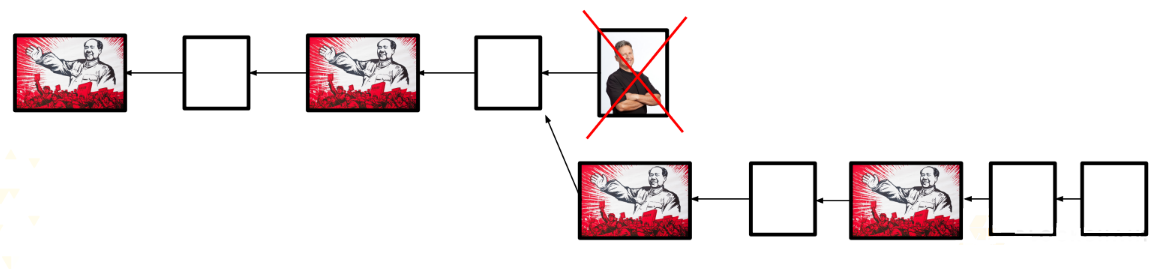
\includegraphics[scale=0.4]{blacklist_feather}
    \end{center}
    
    \section*{Network Attacks --- Timejacking}
    
    Whereas blacklising and malicious mining pool schemes only affect mining profit schemes, it is also possible to create attacks that endanger the entire underlying Bitcoin network. 
    To recap, Bitcoin nodes exchange monetary value through transactions over vast distances and time zones. It becomes a challenge to keep track of time, since it is necessary for each node to in sync with all the other nodes in the network. To address this problem, nodes maintain an \textbf{internal clock time}, which is the median clock time of all its peers. If a node's internal time differs by more than 70 minutes from the local system time, the node reverts its internal clock time to the system time. Additionally, as a precaution, nodes reject new blocks with timestamps that are more than 2 hours ahead of its internal clock.
    
    As an attacker, Alice wants to put a Bob's node out of sync with the rest of the network in order to give herself more time to mine a secret chain and double spend on a target node. To do this, Alice can launch a sybil attack against Bob and every other node. Alice aims to set Bob's internal clock time to be 70 minutes behind the system clock time. For every other node, Alice wants to set the internal clocks 70 minutes ahead of the system clock time.
    
    With these prerequisites fulfilled, Alice can now launch a \textbf{timejacking attack}. This involves mining a new block with a timestamp set 190 minutes ahead of the real time. It is important to set the timestamp to be 190 minutes ahead of the real time because blocks have a 120 minute timeframe during which they are considered valid. Every other node would accept the block, since it is within 120 minutes of their time ($190 - 70 = 120~min$.) Meanwhile, Bob rejects the block, since it is past the 120 minute validation bound. The result is that Alice has effectively partitioned the network, since Bob thinks every new block is invalid, while the rest of the network continues on.
    
    Assuming that Alice can keep timejacking Bob, Alice has an indefinite amount of time to secretly mine blocks for a double spend attack. Alice can then broadcast these blocks to Bob, who thinks it is an alternate chain of history, and then accept them, not knowing that they are in fact invalid blocks. Bob would then send goods over while Alice would not have to spend any real bitcoin. However, for Alice to keep timejacking Bob in order to double spend, she would require a non-trivial amount of hash power to maintain the timejack. Even with a restricted time window however, Alice would still get 70 minutes, or 7 confirmations worth of time, to mine on her double spend chain --- plenty of time for Bob to get tricked and accidentally send goods over in exchange for Alice's fake money.
    
    \section*{DoS Attack --- Malicious Miners}
    
    It turns out that malicious miners can also use timejacking to take down competing miners. They could effectively take the competing miners out of the network and thus increase their own effective hash power. This strategy also works for any type of \textbf{denial of service attack (DoS attack)}. Malicious miners that shut down competing miner's connection to the network can gain effective hash power and thus expect more profit. Taking this one step further, miners with access to a distributed Botnet have a competitive advantage over other normal miners.
    
    \section*{Transaction Malleability}
    
    A consequence of using the cryptographic signature schemes that it does, Bitcoin is also vulnerable to attacks involving \textbf{transaction malleability}. Nodes relaying a fresh transaction can actually tweak certain fields in the transaction to make a version of the transaction with a different hash image, but the digital signature still verifies. For example, in ECDSA, the following signature pairs are equivalent:
    
    $$(r,\textbf{s}~(mod N)) ~and~ (r, \textbf{-s}~(mod N))$$
    
    Both validate the same transaction data, but because they are different values, they have different hash images. Additionally, the scriptSig field can (sometimes) have extraneous script operations tacked on the end. These do not change the functionality of a transaction, but change their hash value.
    
    Transaction malleability is a huge issue because in certain situations, transactions rely on a chain of previous transactions. These types of transactions are common in micro payments, and in the Lightning Network, which we will describe in a later note on scaling the Bitcoin network. Changing the hash image of a prior transactions in a chain of transactions invalidates every subsequent transaction.
    
    Historically, there have been several incidents involving transaction malleability. The most famous is one attack on Mt. Gox: an attacker made withdrawals and Mt. Gox saw what was going on. The attacker used transaction malleability to change the transaction hash during the withdrawal, causing Mt. Gox to think that the transaction did not go through. Meanwhile, the bitcoin was actually sent to the attacker. In the end, Mt. Gox did not deduct the stolen amount from the attacker's account because they could not prove that a transaction had taken place without the right transaction hash. In the end, the attacker basically got free bitcoin from Mt. Gox. 
    
    SegWit (Segregated Witness) is a fix for Bitcoin that solves the problem of transaction malleability. It stores transaction signatures in a separate merkle tree. We will discuss more about SegWit in the scalability note.
    
    
    \section*{Conclusion}
    
    In this section, we will make some broad generalizations about the Bitcoin network and attempt to arrive at a profound conclusion. First, we have to accept the notion that computational power requires electricity, which requires money. Computational power will reach equilibrium if miners break even or are making profit, since mining is such a competitive process. Thus, we can establish that:
    
    \begin{itemize}
        \item Lemma 1: Mining Reward = Mining Cost
    \end{itemize}
    
    If you are roughly breaking even with the capital you invest, there is little to no marginal cost to getting more hash rate.  If you have really efficient hardware, there is negative marginal cost to getting more hash rate. All it takes to obtain 51\% of the network hash rate is to get a lot of capital. This would mean that the ccost of acquiring 51\% network hash power is zero or negative, which is less than the mining cost:
    
    \begin{itemize}
        \item Lemma 2: Cost of acquiring 51\% < Mining cost
    \end{itemize}
    
    After owning more than 51\% of the network hash rate, you have a lot of power. You could crash the currency by doing a bunch of double spends, and then regain this value (and then some) by launching a gold finger attack. You also effective own 100\% of the mining reward. You could just mine only on your own blocks, and since you will always produce the longest proof-of-work chain, all the block reward belongs to you. You can also prevent anyone else from mining using blacklisting via punitive forking. Owning a significant amount of hash rate would also affect the price of bitcoin. If you own 51\% of the network hash rate, then that means 49\% of blocks are orphaned. If you own 80\% of the network hash rate on the other hand, only 20\% of blocks would be orphaned. To the average Bitcoin user, this would not really be an issue, and they would be able to make transactions as usual. Because you get so much power from owning 51\% of the network hash rate, then we can establish:
    
    \begin{itemize}
        \item Lemma 3: Value of 51\% attack > Mining Reward
    \end{itemize}
    
    Combining all three of these lemmas we have established, we can come to the conclusion that the value of a 51\% attack is greater than the cost of acquiring the 51\% hash rate in the first place. Game theory says that 51\% attacking Bitcoin \underline{is profitable}. Bitcoin's underlying assumption that no one will get 51\% of the network hash rate is actually profitable, so what is stopping anyone from doing this?
    
    \section*{Generalization of Vulnerabilities}
    
    Currently, there are a lot of orphaned blocks due to pool wars and other malicious mining strategies. A possible way to offset the costs caused by mining pools is to create insurance contracts for bitcoin stakeholders based on the number of orphaned blocks that are detected. Orphaned blocks let us know that pool wars are probably happening somewhere, and that a miner is being excluded. The concept of exclusion derives from the concept that in general, Bitcoin mining is zero sum. To increase your earnings past your fair share, another miner needs to be excluded, wasting their computational power. 
    
    Suppose miners join a collusion until 80\% of the network hash rate is included, and then exclude the rest of the network, meaning that they do not mine on any blocks that are not created by the collusion. There would be no incentive not to join. If the attack succeeds, then everyone involved gets an increased reward. Additionally, the attack would not fail: the collusion could conduct the attack in such a way that it would not start excluding other blocks until the threshold of 80\% is reached. With these points in mind, Game Theory dictates that there would be no incentive not to join. As a naive example, consider the current day. All it takes to conduct such an attack would be for three or more large mining pools to collude; they would then own more than 51\% of the network hash rate. They could potentially ignore every 10th block of another pool in attempts to increase their own power in the network. Such an attack would be practically undetectable, since blocks are found every 10 minutes, and because it is hard to make any statistically significant, detectable changes. Such a strategy would be more profitable than honest mining strategies. Miners are primarily incentivized by profit, so the question is not whether or not this sort of attack has happened before, but: how many of these secret attacks are going on today?
    
    \section*{Post-Block Reward Bitcoin}
    
    As a recap, the Bitcoin block reward halves every 4 years, and by the year 2140, all bitcoin to ever exist will have already been mined. To further comment on the viability of Bitcoin post-block reward, let us analyze the case of an average future Bitcoin user, who holds \$100,000 in Bitcoin, and is willing to pay \$1,000 in fees. To determine the Bitcoin network security, we have to look at mining incentives, since it is mining competition that creates new valid blocks. The amount of hash power that goes into Bitcoin is dependent on mining reward, and as the block reward diminishes to zero, money must move. Miners must be paid in transaction fees so that they can collect is as mining reward --- incentive to uphold the health of the network. If mining reward is based solely on transaction fees in the absence of block reward, is mining still sustainable? 
    
    $$\frac{\textit{average fees paid}}{\textit{average holdings}} = \frac{\textit{cost of attacking}}{\textit{market cap}}$$
    
    Average fees paid and average holdings are our previously assumed values of \$1,000 and \$100,000, respectively. The cost of attacking is the amount of security and mining power that is being invested in the network. Market cap is the market cap of Bitcoin when the maximum of 21 million BTC has been mined. From this proportion, we can deduce that an attacker only needs to pay 1\% of the market cap of Bitcoin in order to attack. One potential solution to this frightening result would be to increase the velocity of money in Bitcoin. By increasing the speed at which transactions are confirmed and included, miners can add more transactions to their blocks to earn more of the transaction fees. To achieve this, changes to the Bitcoin protocol, such as adoption of the Lightning Network, to boost transaction velocity must be made.
    
    
    
    
    
    % BEGIN KEY TERMS
    \newpage
    \thispagestyle{firstpage}
    \vspace*{2\baselineskip}
    \section*{Key Terms}
    \noindent A collection of terms mentioned in the note which may or may not have been described. Look to external sources for deeper understanding of any non-crypto/blockchain terms.
    \begin{enumerate}
        % edit within here
        \item \textbf{VOCAB WORD} --- Definition. % format
    \end{enumerate}
    % END KEY TERMS
\end{document}